\chapter{Traitement du Langage Naturel}

Après avoir décrit les principes de l'apprentissage par un réseau de neurones, voyons comment on peut les mettre en œuvre. On se restreint à des problèmes impliquant du texte, et plus précisément les problèmes de traitement automatisé du langage naturel. Explorons deux aspects complémentaires de l'apprentissage automatisé, que sont la classification et la génération de textes\footnote{Ces problèmes se retrouvent le plus souvent mis en lumière avec le traitement d'images, mais de récentes expérimentations ont permis à des équipes de chercheurs d'imiter le style d'écriture d'une journaliste. Le succès fut tel que la technologie employée a été gardée secrète, car jugée trop dangereuse si employée à mauvais escient. \url{https://www.theguardian.com/commentisfree/2019/feb/15/ai-write-robot-openai-gpt2-elon-musk}}.

Pour les tâches d'apprentissage, on suppose que chaque auteur écrit dans un style qui lui est propre, reconnaissable par une machine. Le but secondaire de ce projet a été de vérifier cette hypothèse, sachant que le but principal était de découvrir l'apprentissage profond.

\section{Les données}
Nous avons souhaité découvrir les possibilités offertes par l'apprentissage profond pour des données textuelles. Pour ce faire, nous avons construit un corpus de plus de 150 romans de la littérature française classique, dont les auteurs sont Balzac, Dumas, Hugo et Zola (en plus des "Aventures de Télémaque" de Louis Aragon et de "L'Atelier de Marie-Caire de Marguerite Audoux, volontairement incorporés pour perturber les données). Bien évidemment, d'autres auteurs sont envisageables, mais ceux-ci ont l'avantage d'avoir été prolixes : plus de 80 romans pour Balzac, plus de 50 pour Zola; Hugo et Dumas en ont écrit moins, mais très volumineux.

Nous avons utilisé des ressources libres pour récupérer les fichiers texte, à savoir gutenberg.org ainsi que wikimedia.org. Ces sites internet reproduisent de très nombreuses œuvres de manière numérique. Toutefois, il a fallu extraire chaque texte à la main, car, sur le premier site, toute navigation automatisée est interdite, alors que le second site n'a pas une structure suffisamment régulière d'un livre à l'autre pour le faire autrement. Dans une moindre mesure, nous avons aussi ôté toutes les annotations, remarques et certaines parenthèses des textes. Les explications de l'auteur ou de l'éditeur rompent le fil narratif de l'œuvre, en plus d'introduire des caractères spéciaux comme "[". Tous les textes ainsi copiés et pré-traités sont ensuite regroupés par auteur dans un répertoire "textes bruts".

En parcourant les romans écrits par chacun des auteurs cités, on remarque des cas atypiques. Le plus flagrant est "Han d'Islande", écrit par Victor Hugo. Ce roman regorge de mots et de phrases en islandais. Bien sûr, pour le lecteur, tout est traduit en note de bas de page ou entre parenthèses. Cependant, il serait mal venu d'utiliser ce (long) texte pour un algorithme cherchant à reconnaître un auteur. D'une part, enlever toutes les annotations serait à faire manuellement. D'autre part, le corpus se compose d'auteurs classiques français. Pour peu qu'on cherche à construire une représentation sémantique des mots du corpus, on trouverait tout à coup des termes étrangers synonymes de termes français; typiquement une erreur de surinterprétation dans notre cas.

Les deux tâches d'apprentissage utilisent les textes différemment. Pour la génération de texte, il suffit de prendre un texte suffisamment long et le passer à l'algorithme. Nous en décrirons le processus en dernier. Pour ce qui est de la tâche de classification, présentée en premier, il a fallu découper les textes bruts. Leur taille initiale varie entre 20 Ko et 3 Mo, ce qui est très déséquilibré. On emploie alors un script python pour découper les textes en extraits de 300 mots environ. Ce script se charge aussi de labelliser chacun des extraits avec le nom de son auteur. En voici un exemple :

\noindent "hugo

\noindent L'équipage était occupé à enverguer les voiles. Le gabier chargé de
prendre l'empointure du grand hunier tribord perdit l'équilibre. On le
vit chanceler, la multitude amassée sur le quai de l'Arsenal jeta un
cri, la tête emporta le corps, l'homme tourna autour de la vergue, les
mains étendues vers l'abîme; il saisit, au passage, le faux marchepied [...]
"


\section{Classification de textes}
Le code source du classifieur est disponible à l'adresse \url{https://colab.research.google.com/drive/1NZ1NrFBn2ArlpgkgI0PPFFQ0Mu0hZk0n}. Ce code et fourni par Google dans un guide dédié à la classification de textes. Par ailleurs, ce guide comporte une recette pour choisir le meilleur modèle en fonction de quelques critères des donneés. La figure \ref{fig:classif_flowchart} le reproduit.

\begin{figure}
\centering
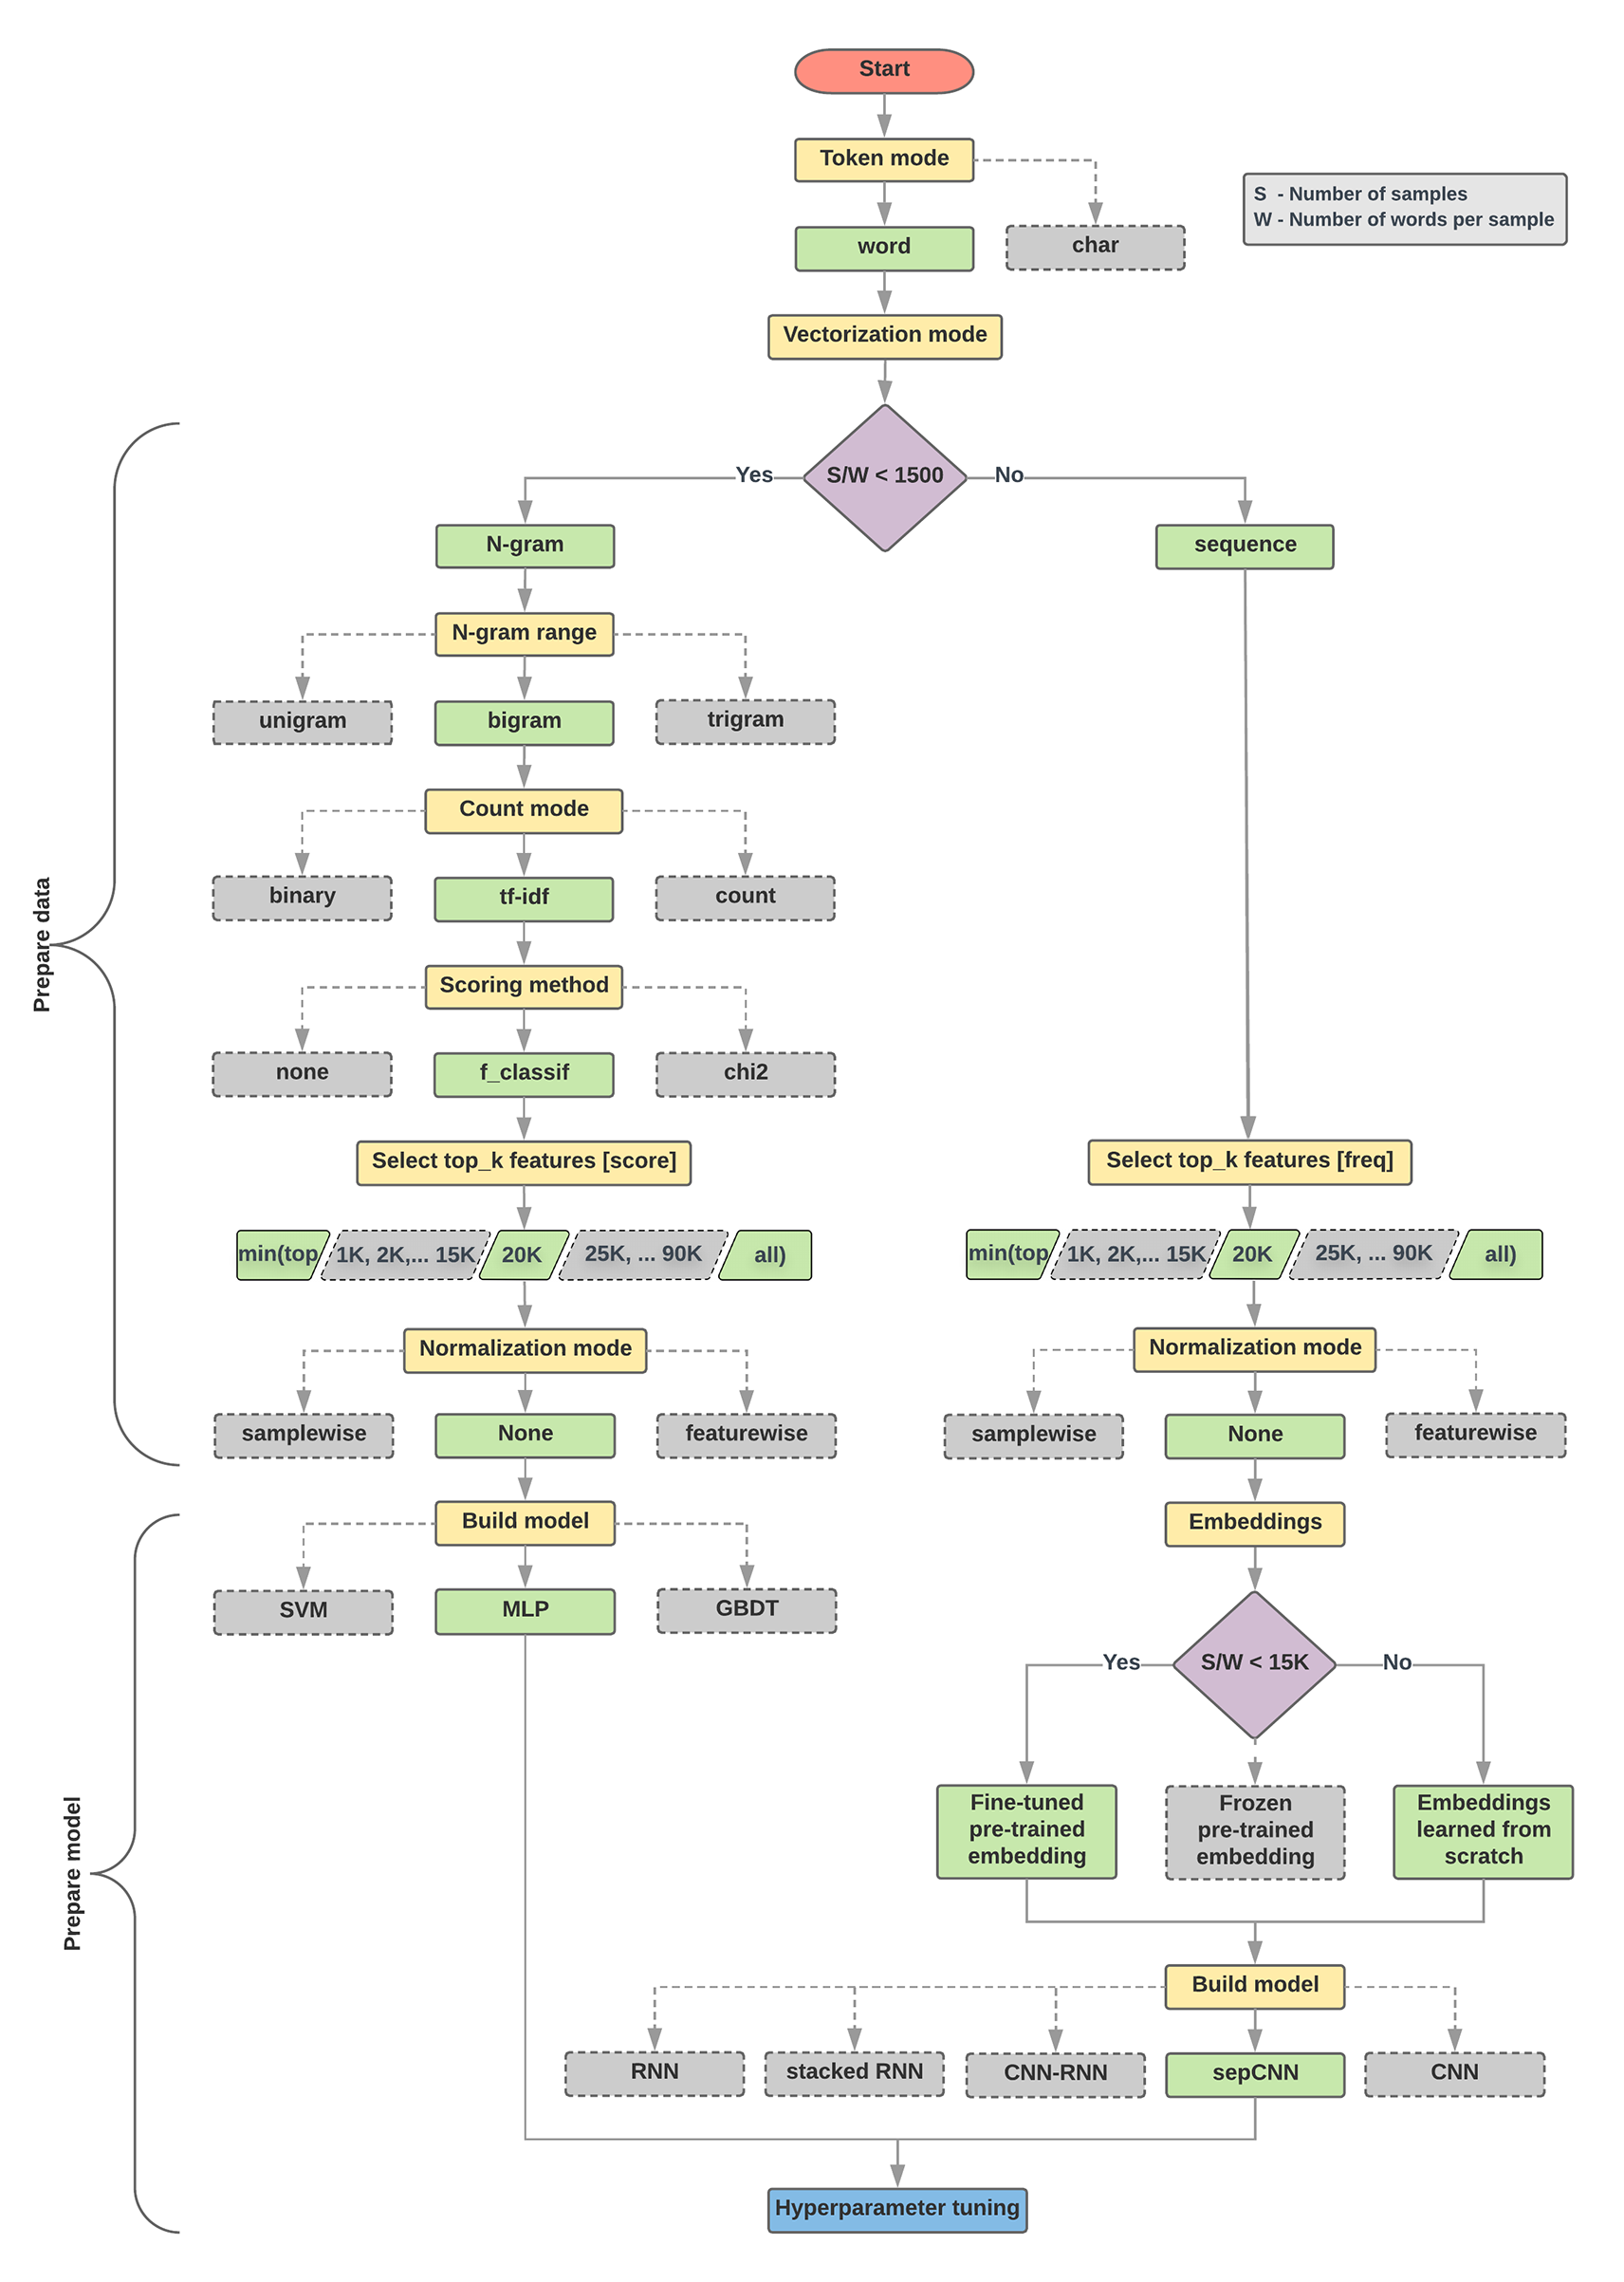
\includegraphics[width=\textwidth]{img/classif_flowchart.png}
\caption{Recette pour un classifieur de textes}
\label{fig:classif_flowchart}
\end{figure}

\subsection{Classification binaire : Balzac ou bien Zola ?}
Voyons tout d'abord une simple classification binaire, dont le but est de déterminer si un extrait a été écrit par Balzac ou bien par Zola.

Voici quelques indicateurs concernant les extraits :
\begin{itemize}
\item Nombre de textes : 16651 (entraînement) + 5551 (tests)
\item Nombre de classes : 2
\item Nombre de textes d'entraînement dans chaque classe : 7817 (Balzac) et 8834 (Zola)
\item Nombre de mots par texte : environ 350
\end{itemize}

Voici les mots les plus utilisés dans les textes d'entraînement (figure \ref{fig:classif_bin_unigram}) : 

\begin{figure}[H]
\centering
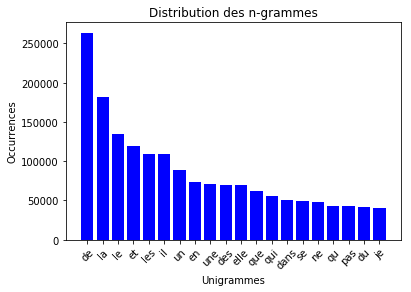
\includegraphics[width=.75\textwidth]{img/classif_bin_unigram.png}
\caption{Occurrences des premiers unigrammes, classification binaire}
\label{fig:classif_bin_unigram}
\end{figure}

Sans surprise, les mots les plus utilisés du texte ne sont pas vraiment porteurs de sens. A eux seuls, il est impossible de reconnaître qui que ce soit.

Il y a 16651 fichiers dans le jeu d'entraînement, chacun comportant environ 350 mots. Le rapport (nombre de fichiers)/(nombre de mots par fichier) est de 47. En suivant les recommandations du tutoriel Google, on choisit de représenter  les données par bigrammes, qui portent plus de contexte que les unigrammes. Ensuite, on les transmettra à un perceptron multicouches simple (comparable à celui de la figure \ref{fig:ffnn}).

Puisque le problème est ici une classification binaire, il est conseillé de choisir une fonction d'activation sigmoïde pour la couche de sortie, ainsi qu'une fonction de perte d'entropie croisée. Voyons alors comment notre réseau réagit face à la tâche demandée :

\begin{figure}[H]
\centering
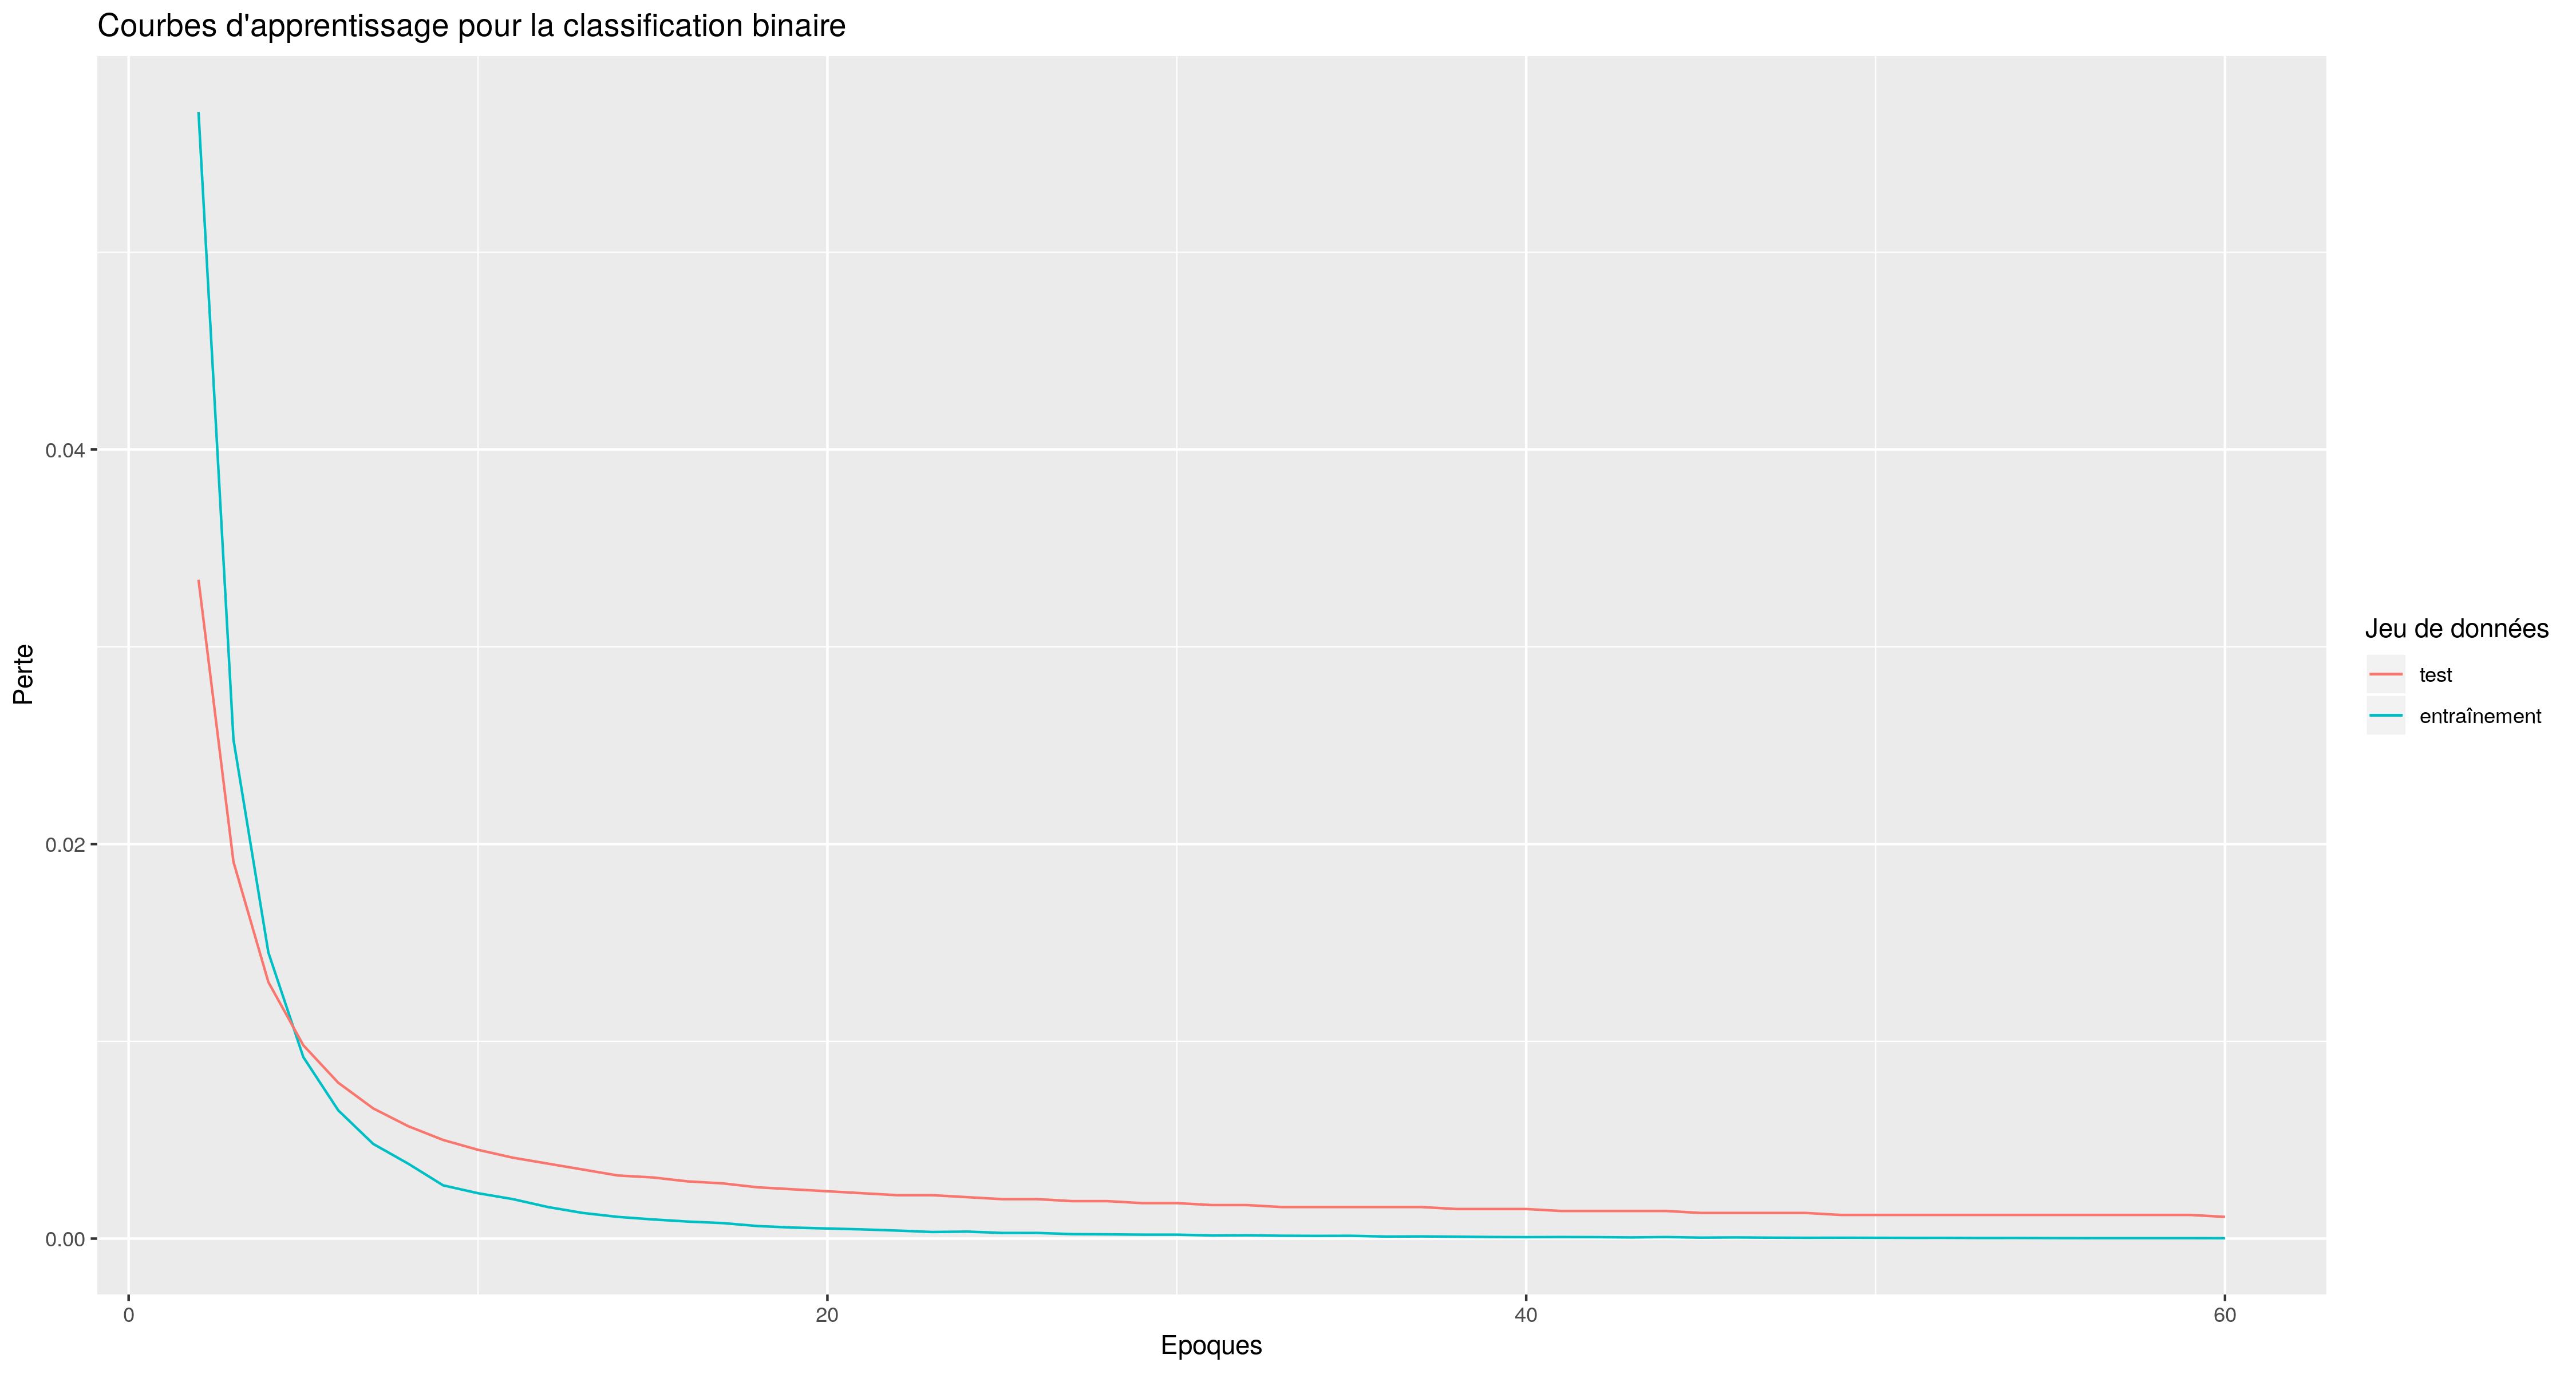
\includegraphics[width=\textwidth]{img/classif_bin_perf.png}
\caption{Courbes d'apprentissage, classification binaire}
\label{fig:classif_bin_perf}
\end{figure}

L'interprétation est claire : le score d'apprentissage est excellent, et le score de test le suis de très près. Aucun signe de mauvais ajustement ne transparaît. De manière assez étonnante, ce petit perceptron à deux couches est capable de prouesses. Ceci n'est bien évidemment pas dû au hasard, mais au travail préalable des chercheurs de Google. Nous avons donc, par notre essai, confirmé leurs dires.

A ce stade, tout est encore possible : le classifieur peut tout à fait échouer à distinguer 5 classes. Voyons ce qu'il en est.

\subsection{Classification multiple : quel auteur ?}
Dans cette partie, on complexifie le problème : partant du corpus entier d'extraits, on tente de faire apprendre à l'algorithme le style de chaque auteur. Saura-t-il les reconnaître ? On s'appuie donc sur les fonctions définies précédemment dans le code.

De même qu'auparavant, voici les indicateurs-clés pour le texte : 
\begin{itemize}
\item Nombre de textes : 23821 (entraînement) + 5959 (tests)
\item Nombre de classes : 5
\item Nombre de mots par texte : environ 350
\end{itemize}

De même que précédemment, les mots vides de sens ont la cote (figure \ref{fig:classif_mult_unigram}). 

\begin{figure}[]
\centering
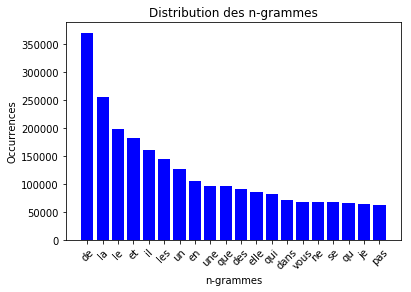
\includegraphics[width=.75\textwidth]{img/classif_mult_unigram.png}
\caption{Occurrences des premiers unigrammes, classification multiple}
\label{fig:classif_mult_unigram}
\end{figure}

En revanche, les classes sont très déséquilibrées les unes par rapport aux autres. La figure \ref{fig:classif_mult_classes} le montre bien; "0" désigne Balzac, "1" Dumas, "2" Hugo, "3" Zola et "4" les autres. Cela pourrait perturber le classifieur. Et même si ce n'est pas le cas, il est conseillé d'équilibrer les jeux de données passés à un algorithme.

\begin{figure}[]
\centering
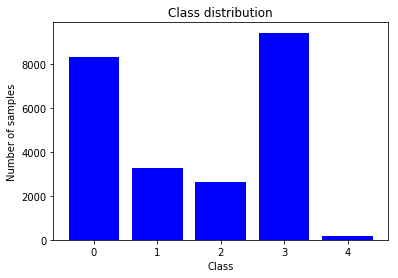
\includegraphics[width=.75\textwidth]{img/classif_mult_classes.png}
\caption{Nombre d'extraits par auteur}
\label{fig:classif_mult_classes}
\end{figure}

Enfin, voyons les courbes de performance pour des classes multiples :

\begin{figure}[H]
\centering
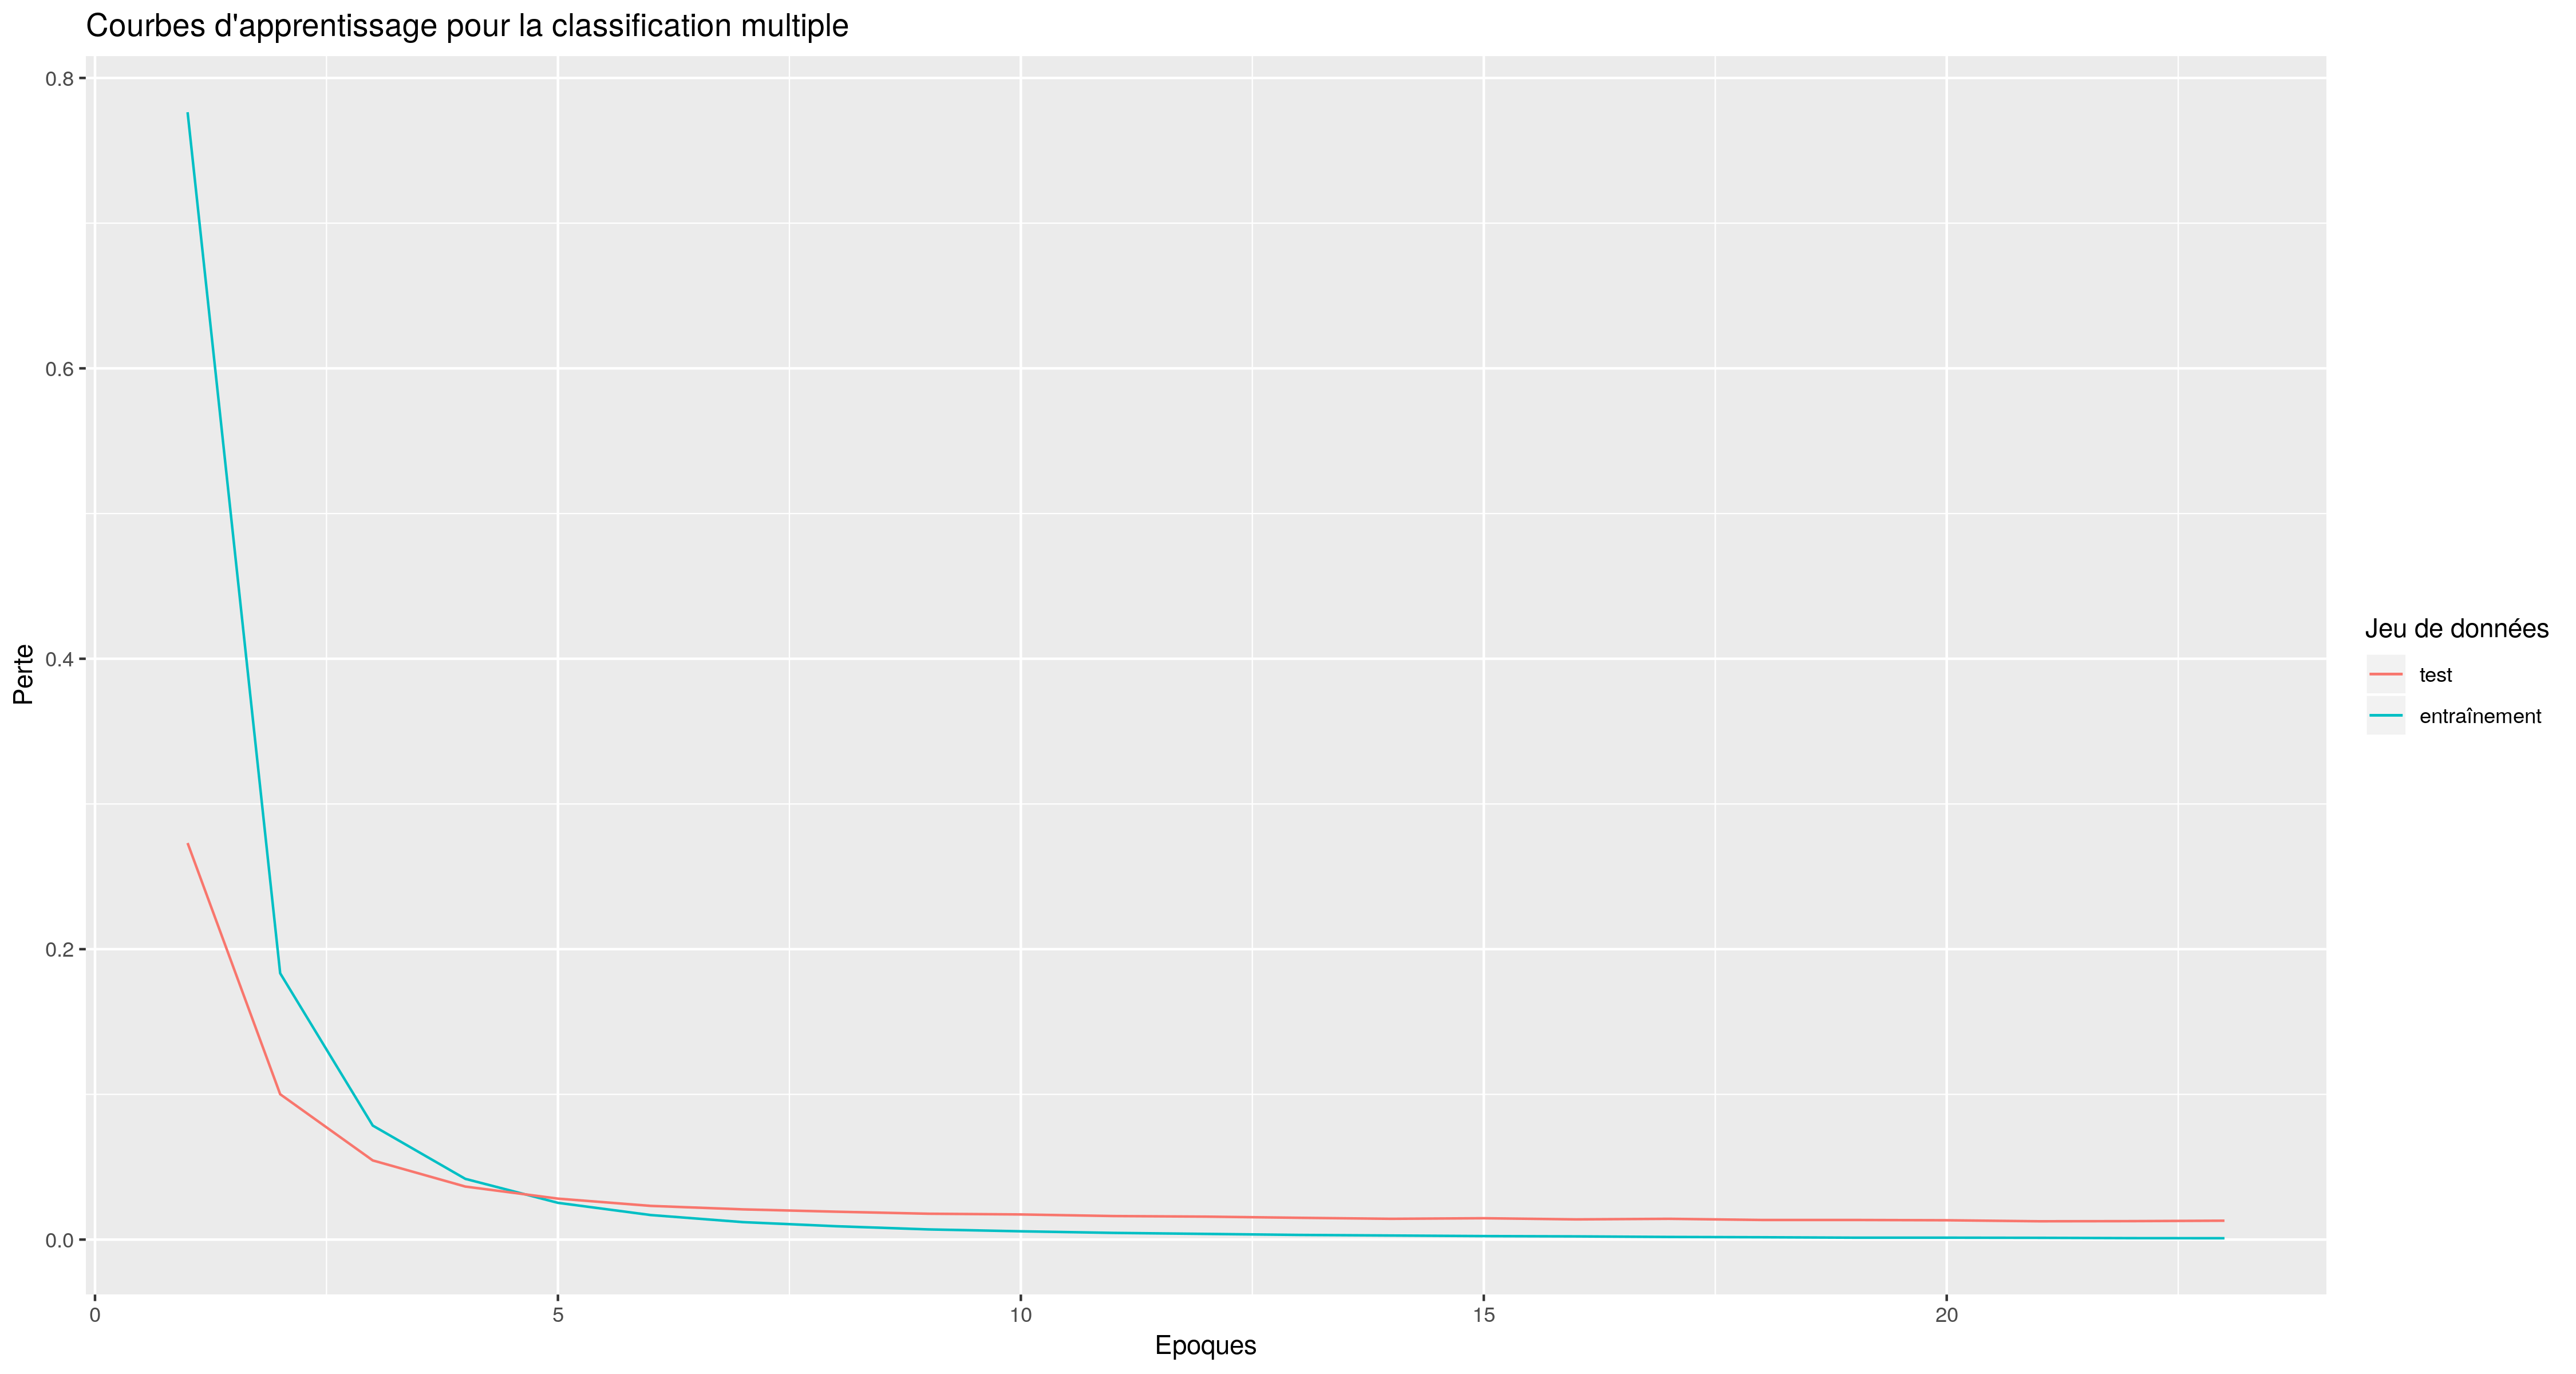
\includegraphics[width=\textwidth]{img/classif_mult_perf.png}
\caption{Courbes d'apprentissage, classification multiple}
\label{fig:classif_mult_perf}
\end{figure}

Sans grande surprise, il semblerait que la recette de Google ait fonctionné une seconde fois. Peut-être que 5 classes par rapport à 2 n'est pas un trop grand effort à fournir pour le réseau. il serait intéressant de voir avec combien de classes il peut travailler avant de faire de mauvais scores.


\subsection*{Conclusion}
Revenons à la problématique. Nous avons certes réussi à distinguer les auteurs entre eux grâce à ce réseau. Néanmoins, est-ce bien le style des auteurs qui a joué ? Plusieurs raisons peuvent nous faire penser que ce n'est pas le cas : le style est une notion abstraite, voire subjective. Également, nous avons utilisé des bigrammes, soit des couples de mots consécutifs, pour entraîner le réseau, mais ceux-ci ne sont pas forcément porteurs de beaucoup de sens. 

La partie suivante va peut-être nous éclairer.

\section{Génération de texte}
Générer du texte après une pahse d'apprentissage est une autre affaire. Ici encore, nous avons repris le code des ingénieurs que nous avons adapté à nos besoins. Il est disponible à l'adresse : \url{https://colab.research.google.com/drive/1W6QNRw-n-vK-iULLNJWsOL8dSCixixlU}

Il y a une difficulté conceptuelle supplémentaire qui est l'architecture particulière du réseau génératif. Le réseau classifieur est dit \emph{à propagation avant}, alors que celui-ci est qualifié de \emph{récurrent}. La motivation vient justement de problèmes comme le nôtre, où les données d'entrée sont des séquences. On fait alors "boucler" le réseau sur lui-même, sortie vers l'entrée. A cela s'ajoute un décalage dans le temps par pas discrets. 

L'architecture de notre réseau est présentée figure \ref{fig:gen_texte_ent}

\begin{figure}[]
\centering
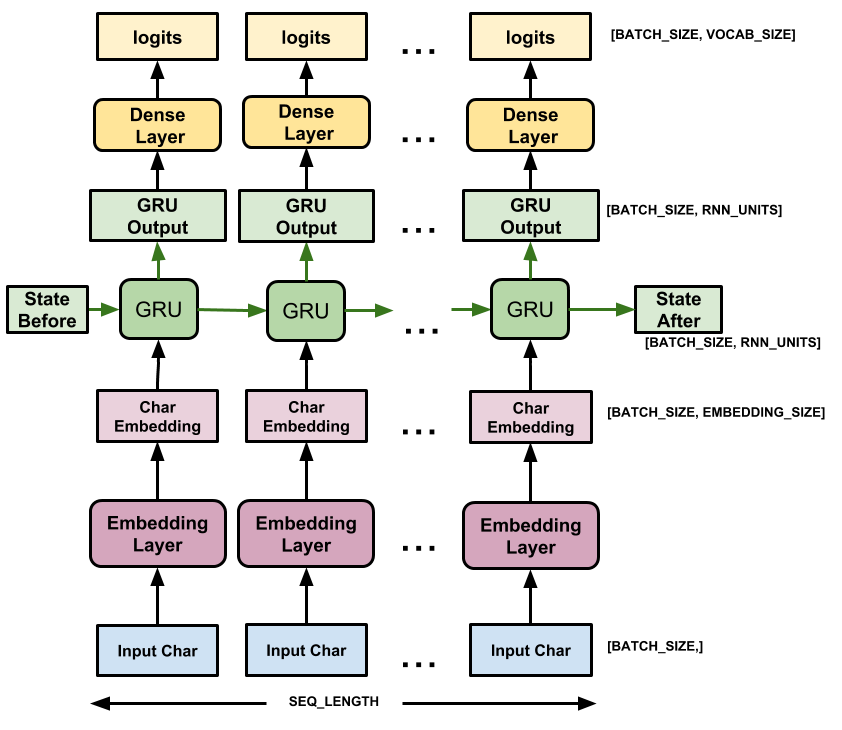
\includegraphics[width=\textwidth]{img/gen_texte_ent.png}
\caption{Vue "dépliée" du réseau récurrent génératif}
\label{fig:gen_texte_ent}
\end{figure}

Ceci donne lieu à la boucle de prédiction suivante : 

\begin{figure}[]
\centering
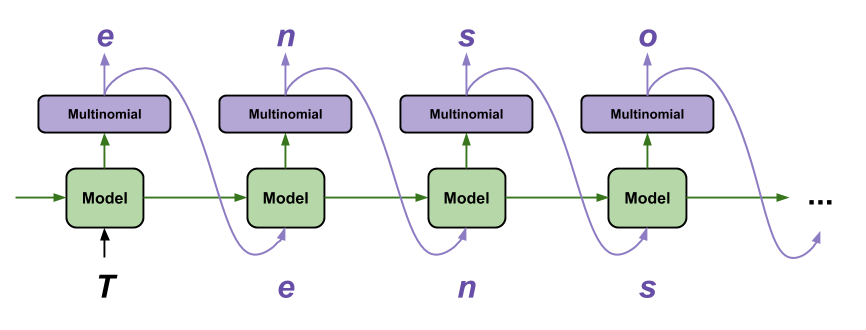
\includegraphics[width=\textwidth]{img/gen_texte_boucle.png}
\caption{Boucle de génération de caractères}
\label{fig:gen_texte_boucle}
\end{figure}

On a entraîné sur Germinal de Zola. Voici ce qu'il génère après 30 époques d'entraînement et à partir de "Monsieur, " : 

\noindent "Monsieur, le derrière, en hâte. Il semblait que tout le coron se tuait de sa taille, pressé d’envoyer la crosse farouche.

\noindent — Veux-tu bien de d’où en les autre, il faut tirer En bas de la cheminée, ils n’en routes pas avec les petits, et quand il eut découdé que deux patients, qu’ils voyaient une décoration, le flaire était achevé de défendre. Il baiserait tout de même potiller. On avait là, fondu entrer, ler maintenant, éternelle moins de toilette, M. Grégoire accrochant de tuerelle, alors, pour l’empêcher de ricaner encore, avec ses deux mères les petits jupes dont les mineurs se méfiant. S’il ne s’y donnait pas sa main, il bégaya :

\noindent — Qu’est-ce que nous avec quatre journées de deux filles ! Le resta que les dragons et lesquelles la délait pas, commençaient à droite et à gardirent : déjà là Répiller, mai tranquillis devant lui, au sombre, lorsque dans l’imple d’orgueil, jusqu’aux petits et ses sabots, bourdonnant dans le panier de la fenêtre. Mais des crânes de faim, tous les journ’approche du "

Et voici ce qu'on obtient après 50 époques :
\noindent "Monsieur, dans un bois en l’air, bravement, se bouchaient d’une grande partie de la foule. Je croyais nous filaient trop haut, au milieu de ces retour sur sa cage. Peut-être ne refusait pas, elle tremblait, on se fâchait. Aussi, chez le porion sur les hieries violentes devaient se tenir famille se laisser en un pal flacon.

\noindent Trois heures sonnaient, l’écrasemort en était avec le commé cette société portant à gravocher la tête aux ongles dehors, le cœur ni les autres baissèsent le solant d’ici, qu’ils n’auraient pas fait de débit en bon ouvrier qui se frit dans le haut évendre encore, avec Mouquet et Levaque, en outrangBarres, qui lui eût empaient sans la fenêtre ; seulement, les hommes, la fille d’un hurlement terché, le reste de ven en était plus la caresse, on retournerait aux guides. Mouquet eut un re, En partant d’excitationsuméraient les camarades en tamaient : à Feutry-noyée ; à Saint-Thomas, où il voulait la Compagnie entendait seul ici farouche.

\noindent Chaval volent se haussait. Quand ils sortir"

La ressemblance avec de vraies phrases se précise, mais surtout à l'échelle de quelques mots consécutifs. Après tout, c'est sur des séquences correctes de mots que le modèle a été entraîné.

\section*{Conclusion}
D'une part, nous savons maintenant qu'il est possible de reconnaître au moins 5 auteurs différents grâce à des extraits de leurs œuvres. ous savons aussi qu'en entraînant un réseau de neurones récurrent, il est possible de générer du texte de plus en plus réaliste. Mais par contre, nous ne pouvons pas affirmer grand chose quant au \textit{style} d'écriture. Les bigrammes du classifieur ne l'ont sans doute pas capturé. Et ce n'est visiblement pas encore le cas du réseau récurrent. Finalement, d'autres recherches s'imposent.